\begin{figure}[t]
  \centering
  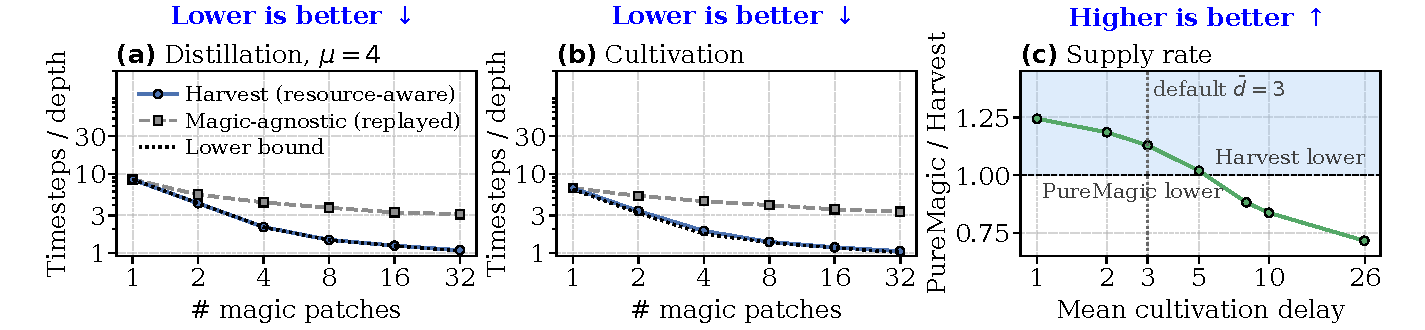
\includegraphics[width=\linewidth]{figures/evaluation/fig_rq4_supply.pdf}
  \caption{\textbf{Magic-state protocols} (RQ4). Timesteps over the critical path as the number of magic-state patches grows under \textbf{(a)}~distillation with $\mu=4$, \textbf{(b)}~distillation with $\mu=10$, and \textbf{(c)}~cultivation. Harvest schedules against the supply model; the magic-oblivious schedule is computed for instant supply and replayed with stalls. The dotted line is the lower bound $\max(T_{cp}, \text{supply})$. Panel titles give the number of circuits.}
  \label{fig:rq4-supply}
\end{figure}
